\documentclass[a4paper,10pt]{book}
\usepackage{MyMathematicalUniverse}



\title{My mathematical universe}
\author{Haoran Li}
\date{}



\RequirePackage[
    backend=biber,         % Use Biber as the backend
    style=alphabetic,      % Alphabetic citation style (you can change this)
    sorting=ynt            % Sort by year, name, and title
]{biblatex}
\addbibresource{Bibliography.bib}



\makeindex[columns=2, title=Index, intoc] % Create the index



\begin{document}\sloppy % Reduce overlong words



% Maketitle
\begin{titlepage}
\begin{center}
\vspace*{1cm}
\Huge
\textbf{My Mathematical Universe} \\
\vspace{1cm}
\Large
Haoran Li \\
\vspace{3cm}
\begin{center}
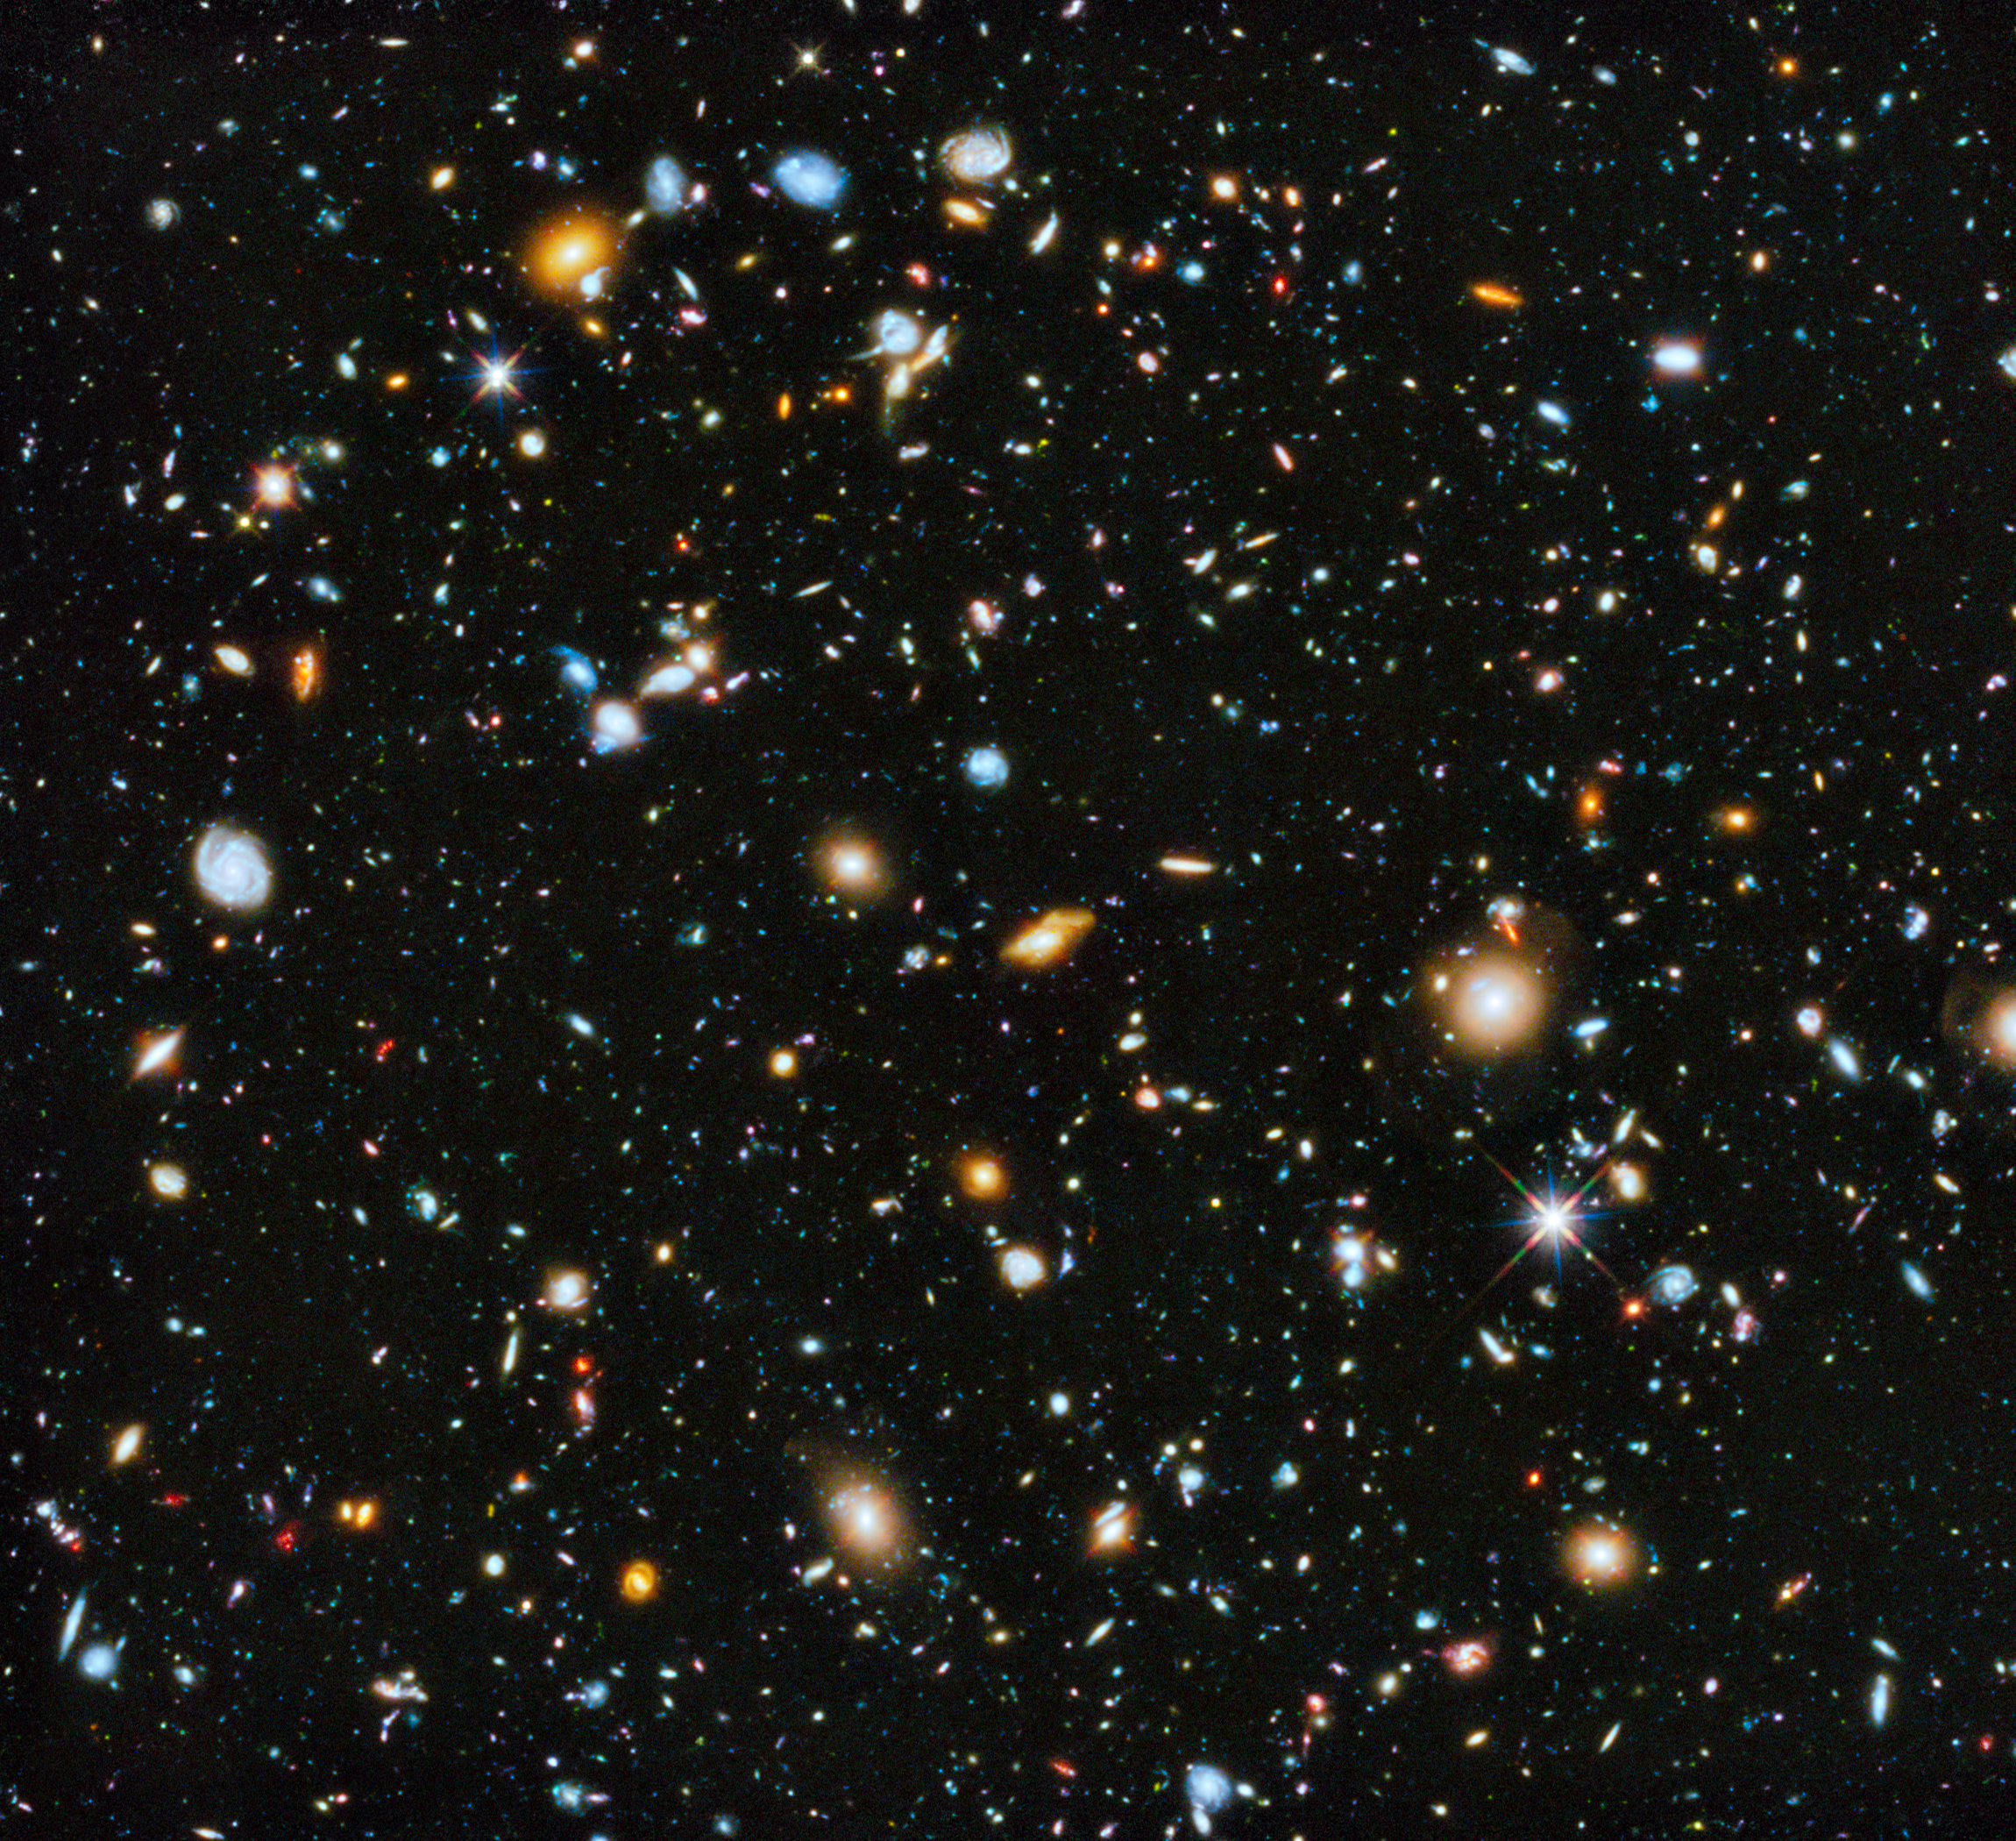
\includegraphics[width=0.7\textwidth]{Pictures/Universe.jpg}
\end{center}
\end{center}
\end{titlepage}



\tableofcontents
\let\tableofcontents\relax
\newpage


\chapter{Category theory}
\subfile{CategoryTheory.tex}
\begin{center}
\includegraphics[width=0.5\textwidth]{Pictures/Alexander_Grothendieck.jpg}
\end{center}
\newpage



\chapter{Partial Differential Equation}
\subfile{PartialDifferentialEquation.tex}
\newpage







\printindex



\end{document}